\begin{itemize}
    \item {\itshape First Law} (Law of Inertia): In the absence of external forces, a particle moves with a constant velocity. This law holds even in frames accelerating near the speed of light, $c$. An inertial frame is defined by where the first law holds. The relationship between different inertial reference frames is called the Lorentz transformations.
    
    \item{\itshape Second Law} (Equation of Motion): For any particle of mass $m$, the net force $F$ on the particle is always equal to the mass times the particle's acceleration. Mathematically, $\vec{F} = m \vec{a}$. Rephrased to the particles momentum, $\vec{p} = m \vec{v}$.
    
    This notation can be simplified using dot notation: $n$ dots above a function of t represents the $n$-th derivative of that function with respect to time. Therefore, $\vec{F} = \dot p = m \vec{a} = m \dot v$.
    
    Newton's second law yields differential equations very often, most of which are quite easy to solve. See example 2.2 for a true example. For a watered-down version,
    
    \begin{equation*}
        \ddot x(t) = \frac{F_0}{m}.
    \end{equation*}
    
    \noindent Where $F_0$ is some contant applied force and $m$ is the particle mass. To solve, just integrate each side twice,
    
    \begin{equation*}
        \int \int \ddot x(t) dt = \int \int \frac{F_0}{m} \rightarrow \int \dot x(t) = \int \frac{F_0}{m}t + v_0 \rightarrow x(t) = \frac{F_0}{2m}t^2 + v_0t + x_0.
    \end{equation*}
    
    Classical mechanics often delivers problems in the form of differential equations, so it is important to be able to solve them, and solve them quickly for the GRE.
    
    \item{\itshape Third Law} (Reactionary Forces): If an object 1 exerts a force, $F_{12}$, on an object 2, then object 2 exerts it's own force, $F_{21}$ (a reactionary force), on object 1. These two forces are equal in magnitude and opposite in direction. That is, $\vec{F}_{12} = -\vec{F}_{21}$.
    
    Additionally, when these forces act along a straight line between their centers of mass, these reactionary forces are called {\bfseries central forces}. An example of this is the gravitational forces between celestial bodies.
    
    The third law is closely related to the conservation of momentum. It is proven below that the total momentum of any multiple-particle system is constant, as long as there are no external forces. Mathematically, if $\vec{F}_{ext} = 0$, then $\vec{p} = const.$
\end{itemize}


% --- EXAMPLE: MOMENTUM WITH 4 PARTICLE SYSTEM
{\exbegin Example 2.1: Momentum in a 3-particle system}

Imagining a three particle system such as the one shown in figure \ref{fig:three-part-sys}, it can be shown that the system observes (roughly) the conservation of momentum. A system like this could be a sun-planet-moon system with an outside force such as a massive invading spaceship. Any of these three objects has three total forces acting on it:

\begin{figure}
    \centering
    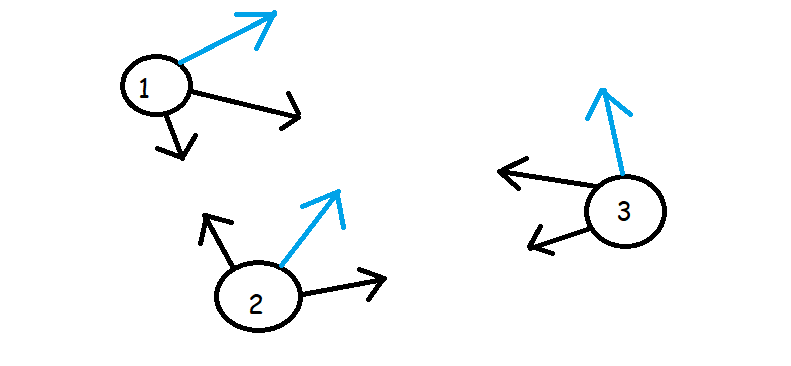
\includegraphics[width=10.5cm]{Classical_Mechanics/2.2-Newton/three-particle-sys.png}
    \caption{A three particle system. The blue arrows represent an external force, while the black represent the internal forces of the system.}
    \label{fig:three-part-sys}
\end{figure}

\begin{align}
    \text{(net force on 1) } \vec{F_1} = \vec{F}_{12} + \vec{F}_{13} + \vec{F}_1^{ext} \\
    \text{(net force on 2) } \vec{F_2} = \vec{F}_{21} + \vec{F}_{23} + \vec{F}_2^{ext} \\
    \text{(net force on 3) } \vec{F_3} = \vec{F}_{31} + \vec{F}_{32} + \vec{F}_3^{ext}
\end{align}

\noindent The rates of change of these particles' momenta using Newton's second law is,

\begin{align}
    \label{eqn:momentums}
    \dot \vec{p}_1 = \vec{F_1} = \vec{F}_{12} + \vec{F}_{13} + \vec{F}_1^{ext} \\
    \dot \vec{p}_2 = \vec{F_2} = \vec{F}_{21} + \vec{F}_{23} + \vec{F}_2^{ext} \\
    \dot \vec{p}_3 = \vec{F_3} = \vec{F}_{31} + \vec{F}_{32} + \vec{F}_3^{ext}.
\end{align}

\noindent Now, defining the total momentum of our system as $\vec{P}$, then the rate of change, $\dot \vec{P} = \dot \vec{p}_1 + \dot \vec{p}_2 + \dot \vec{p}_3$. Adding all of equations \ref{eqn:momentums}, 5, and 6 will yield a result $\dot \vec{P} = \vec{F}^{ext}_1 + \vec{F}^{ext}_2 + \vec{F}^{ext}_3$. This is due to the fact of the third law, that reactionary forces are equal and opposite, such that the forces between the objects cancel out. In the special case that there are no external forces, $\dot \vec{P} = 0$.

{\exend }

The example above can be extended to any number of particle systems. This means that any $N$-particle systems conserves momentum in classical mechanics. The main point to drive home is that internal forces have no effect on the evolution of the total momentum, $P$. $P$ is determined solely by the net external force on the system.

{\bfseries Principle of Conservation of Momentum}: If the net external force, $\vec{F}_{ext}$, on an $N$-particle system is 0, the system's total momentum, $\vec{P}$, is constant. This is an important and useful result in classical mechanics, and, for the most part, holds true in relativistic situations and quantum mechanics. Newton's third law is the equivalent to this principle. 

% ---- EXAMPLE: NEWTON'S 2ND IN CARTESIAN COORDINATES
{\exbegin Example 2.2: Newton's 2nd Law in Cartesian coordinates}

A block sliding down an incline is one of the most common problems in introductory physics. In this example, a block of mass $m$ is observed accelerating from rest down an incline with a coefficient of friction $\mu$ and is at an angle $\theta$. How far will it travel in time, $t$?

\begin{figure}
    \centering
    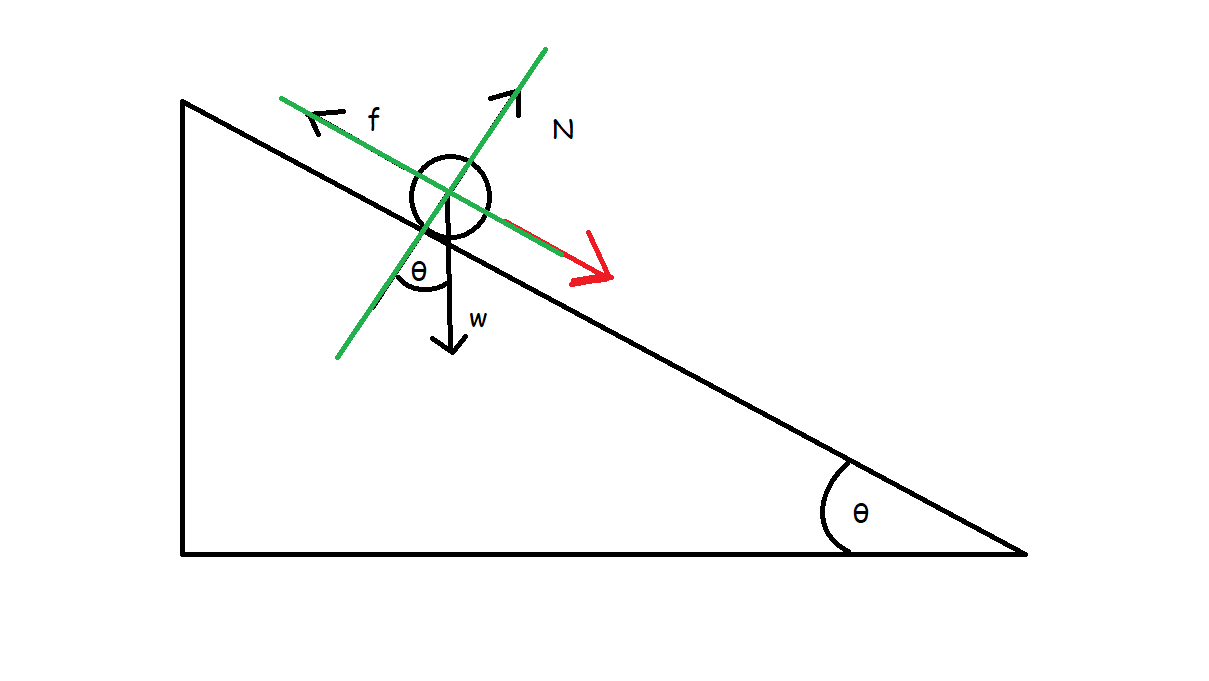
\includegraphics[width=10.5cm]{Classical_Mechanics/2.2-Newton/ball-on-incline.png}
    \caption{The green lines represent the reference frame used in this example and red arrow signifies motion of the ball. Each of the three external forces are labeled.}
    \label{fig:ball-on-incline}
\end{figure}

Choosing the most convenient reference frame, shown in figure \ref{fig:ball-on-incline}, the block is accelerating only in the direction of the x-axis. Friction, $\vec{f}$, is pointed in the negative x-axis and the normal force, $\vec{N}$, is pointed in the positive y-axis. The weight, $\vec{w}$, is known as $m\vec{g}$. 

Applying Newton's second law in both directions gives you,

\begin{align*}
    F_x = m \ddot x - f + w_x \\
    F_y = m \ddot y + N + w_y.
\end{align*}

\noindent Breaking each force into it's components, $f = \mu mg$, $w_x = mg cos\theta$ and $w_y = mg sin\theta$, substituting into the $F_x$ equation, and cancelling the masses,

\begin{align*}
    \ddot x = g(sin\theta - \mu cos\theta).
\end{align*}

\noindent Integrating twice and setting the integration constants to 0 (started from rest and initial starting point was set to be 0 in reference frame), we find,

\begin{equation}
    x(t) = \frac{g}{2} (sin\theta - \mu cos \theta) t^2.
\end{equation}

{\exend }

{\exbegin Example 2.3: Newton's 2nd Law in Spherical Coordinates}

\begin{figure}
    \centering
    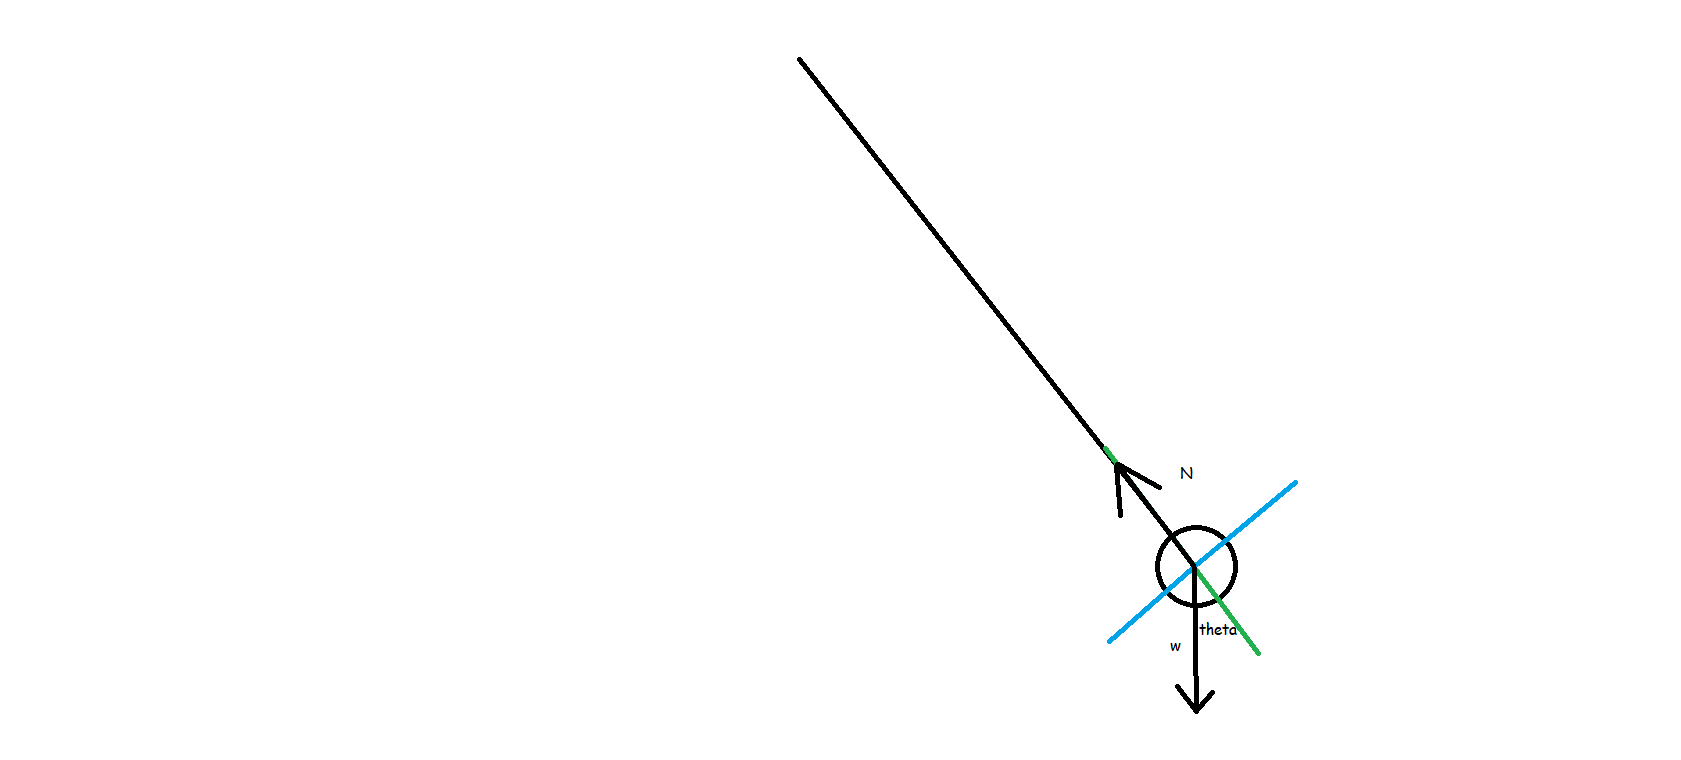
\includegraphics[width=10cm]{Classical_Mechanics/2.2-Newton/ex-pendulum-fig2.png}
    \caption{Sketch of a pendulum and the forces acting upon it.The blue and green lines represent the x and y directions.}
    \label{fig:ex-pendulum-fig}
\end{figure}

In the Miscellaneous - polar coordinates section, the acceleration function of a vector function $ \vec{r}(t) = r\hat{r} $ was derived as,

\begin{equation}
    \label{eqn:polar-coord-newtons-2nd}
    \vec{a} = \frac{d}{dt}[\dot r \hat r] + \frac{d}{dt}[r \dot \phi \hat \phi] \rightarrow (\ddot r - r \dot \phi^2) \hat r + (2\dot r \dot \phi + r \ddot \phi) \hat \phi.
\end{equation}

\noindent This was given as equation \ref{eqn:polar-coord-deriv5} in that section.

The easiest example is one in which $r$ is held constant, such as a pendulum with a fixed length $R$. When equation \ref{eqn:polar-coord-newtons-2nd} is considered for $\dot r = \ddot r = 0$ through Newton's 2nd law,

\begin{equation*}
    \vec{F} = m \vec{a} = m(-R \dot \phi^2) \hat r + m(R \ddot \phi) \hat \phi.
\end{equation*}

\noindent Equating each force component with it's respective unit vector yields,

\begin{align}
    \label{eqn:ex-pend-force-components_r}
    F_r = -mR \dot\phi^2 \\
    \label{eqn:ex-pend-force-components_phi}
    F_\theta = mR\ddot\phi.
\end{align}

The total force radial component is equal to $mg cos\phi - N$ and the total force angular component is equal to $-mg sin\phi$ as seen in figure \ref{fig:ex-pendulum-fig}. Equating equations \ref{eqn:ex-pend-force-components_r} and \ref{eqn:ex-pend-force-components_phi} and those given above,

\begin{align*}
    F_r = mg cos\phi - N = -mR \dot \phi^2 \\
    F_\phi = -mg sin\phi = -mR \ddot \phi
\end{align*}

\noindent Cancelling the $m$'s and and isolating $\ddot \phi$ in the $F_\phi$ equation and, after some rearranging,

\begin{equation}
    \label{eqn:pend-dub-diff}
    \ddot \phi = -\frac{g}{R}sin \phi.
\end{equation}

Equation \ref{eqn:pend-dub-diff} is a difficult second-order differential equation to solve analytically, Luckily, this can be solved with ease using numerical analysis. Figure \ref{fig:pend-solve-fig} shows the solution over a 10 second time span. The attached code {\itshape ex-pendulum.py} shows the Python script to solve this equation.

\begin{figure}
    \centering
    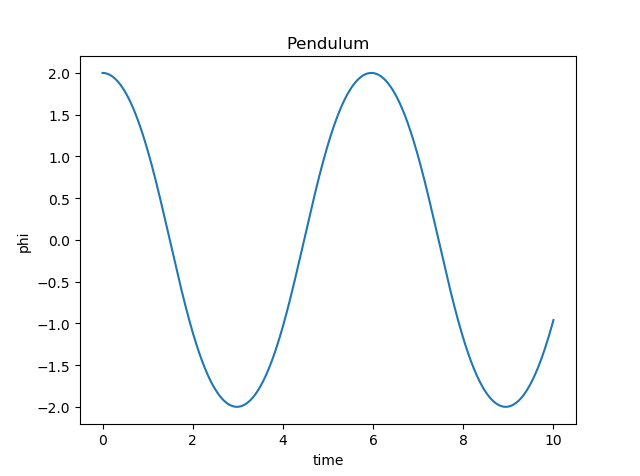
\includegraphics[width=10cm]{Classical_Mechanics/2.2-Newton/ex-pendulum-fig.png}
    \caption{Plot of time (sec) vs. $\phi$ (rad). The cyclical nature of the plot represents the motion of the pendulum.}
    \label{fig:pend-solve-fig}
\end{figure}

{\exend}